\documentclass[a4paper,12pt]{report}
\usepackage{algorithmic}
\usepackage[linesnumbered,ruled,vlined]{algorithm2e}
\usepackage[margin=2cm]{geometry}
\usepackage[utf8]{inputenc}
\usepackage{listings} 
\usepackage{graphicx} 
\usepackage{color}
\usepackage{xcolor}
\usepackage{hyperref}
\usepackage{subcaption}
\usepackage[bottom]{footmisc}
\usepackage{verbatim}
\usepackage{fancyvrb}
\usepackage{amsmath}

%\usepackage{mdframed}

\newcommand{\currentdata}{ 1 February 2017}
\newtheorem{example}{Example}

\begin{document}
\vspace{-5cm}
\begin{center}
Department of Computer Science\\
Technical University of Cluj-Napoca\\

\includegraphics[width=10cm]{fig/footer}
\end{center}
\vspace{1cm}
%\maketitle
\begin{center}
\begin{Large}
\textbf{Structure of Computer Systems}\\
\end{Large}
\textit{Laboratory activity 2019-2020}\\
\vspace{3cm}
Project title: Surveillance System\\
\vspace{1.5cm}
Name: Mateiu Bianca\\
Group: 30434\\
Email: mateiu.bianca@gmail.com\\
\vspace{6cm}
\vspace{1cm}

\includegraphics[width=10cm]{fig/footer}
\end{center}

\tableofcontents

\chapter{Research}

The project I want to develop is an online Surveillance System, that uses the webcam. The functioning is simple: the system processes each frame captured by the camera, and when it detects motion, it reports it. The system will also generate a video file, containing only the parts of the recording that had some sort of movement.

Video surveillance is no new technology, and it has been around for a while. It has proven itslef useful in many sectors of our society, but lately, it has been a significant increase in the development of home securtiy systems. My project was developed with the same purpose in mind.

After some research concerning the available tools and technologies, I have decided to use OpenCV for video processing, and Flask for the Web Application.

\section{OpenCV}
OpenCV was started at Intel, in 1999, and the first release came out in 2000. It supports a wide variety of programming languages, among wich \textit{Python}, which I have decided to use.\cite{wiki01}

Among OpenCV's application areas we can find:\cite{wiki02}

\begin{itemize}
\item facial recognition system
\item gesture recognition
\item human-computer interaction
\item motion tracking
\end{itemize}

We can see that the problem we are dealing with is similar to that of motion tracking, only it is more simplified. Instead to locating and tracking a moving object, we simply have to detect if \textit{something} moved in the scene, and then trigger some actions, such as saving the frames to a video file.

I have installed OpenCV using the package installer for Python, \textit{pip}, by running the command \texttt{pip install opencv-python}

\section{Flask}

Flask is a simple, lightweight WGSI(\textit{Web Server Gateway Interface}) web application framework. \cite{wiki03}, used for building websites in Python. I chose to use this framework to stream the video recorded by the web camera. I have installed it using pip as well, with the command \texttt{pip install Flask}


\chapter{Analysis and design}

In order to create a Video Surveillance System, the first thing we require is, of course, a video camera. For this project, I will be using the Web camera of my laptop, but if the project were to be developed further, an actual security camera would be more suited for the job.

The next step is to access the frames captured by this camera, and we can easily do this using OpenCV. Also using OpenCV, we must compare consecutive frames, and find the difference between them. When this difference is high, we can assume that motion has been found. We will use the standard deviation of the difference between frames, which is is a measure of the amount of variation or dispersion of a set of values.

If motion is detected, than the frame will be written to a '.avi' video file, and saved on the local hard-drive. Also, we can see when the system detects motion beacuse the program will write a text on the video streamed on the Web Application.

In regards of the Web Application, this will have a home page, containing only a button, that will start the Video Surveillance when it is pressed. The pressing of this button also concludes to the generation of a new '.avi' file on the hard drive of the computer, containing the frames that captured movement. When the user clicks the button, he will be redirected to another page, containing the video streaming. This page will also have a button, that will redirect the user back to the home page.


\chapter{Implementation}

The project contains two python files:
\begin{enumerate}
\item camera
\item main
\end{enumerate}

\section{camera.py}

This file contains the declaration of the \textit{VideoCamera} class, that deals with capturing the video, reading and comparing frames, detecting movement and writing the video file containing motion.

The first step is to import cv2, and start the video capturing:

\begin{Verbatim}[frame=single]
    self.cap = cv2.VideoCapture(0)
\end{Verbatim}

This line captures the video stream from camera source, while the parameter, 0, refers to the first camera.

The most important method of this file is \textit{computeDifference}. I will go throught this method line by line, and I will also show through pictures the output of each line:

\begin{Verbatim}[frame=single]
    _, self.frame1 = self.cap.read()   
    gray1 = cv2.cvtColor(self.frame1, cv2.COLOR_BGR2GRAY)

     _, self.frame2 = self.cap.read()
    gray2 = cv2.cvtColor(self.frame2, cv2.COLOR_BGR2GRAY)
\end{Verbatim}



The first step is to read 2 frames, and convert them to grayscale. In picture (a) from \ref{fig:pic1}, we can observe the frame captured by the video camera (without conversion). The reason we convert them to grayscale is beacuse it for the method we will use next to compute the absolute difference between frames, grayscale images are required. 

\begin{Verbatim}[frame=single]
    dist = cv2.absdiff(gray1, gray2)
\end{Verbatim}

The next step, as I said, is to compute the absolute difference between the two images.(See \ref{fig:pic1} picture (b)) The output of this function will be an \textit{intensity image}, an image that will have values between 0 and 1, so it will not be just black and white. So we will use the \textit{threshold} function to obtain a black and white image(\ref{fig:pic1} picture (c)):

\begin{Verbatim}[frame=single]
    _, self.thresholdImg = cv2.threshold(dist, 20, 255, cv2.THRESH_BINARY)
\end{Verbatim}

What this function does is go over every pizel value, and if it is greater than a threshold value (second parameter, 20 in our case), it is assigned one value (white), else it is assigned another value (black). Next, we want to reduce the noise in the image, by applying a filter:

\begin{Verbatim}[frame=single]
    self.thresholdImg = cv2.GaussianBlur(dist, (9, 9), 0)
    _, self.thresholdImg = cv2.threshold(self.thresholdImg, 20, 255, 
                                                           cv2.THRESH_BINARY)
\end{Verbatim}

After applying the filter the output is again an intensity image(\ref{fig:pic1} picture (d)), so we need to apply the threshold function again(\ref{fig:pic1} picture (e)). Lastly, we calculate the standar deviation of the image, and return it(\ref{fig:pic1} picture (f)):

\begin{Verbatim}[frame=single]
    _, stDev = cv2.meanStdDev(self.thresholdImg)
    return stDev
\end{Verbatim}

In the method \textit{getFrame}, which is called from the \textit{main} file, the value returned from the previous method is copared to a treshold deviation chosen by us (the lower the value, the greater the sensitivity of the motion detection system), and if it is higher, than we consider that motion was detected. 

If motion was detected, than write both frames to the video file (so the saved video will look as the streamed one), and write the text: 'REC' and 'MOTION DETECTED' on the image that will be returned from this method, to signal the user that the video is being recorded, and that motion was detected. In order to write text on the frames, we use another method from OpenCV, \textit{putText}.

Lastly, encode the frame to 'jpeg' format, and return it.

\vspace{0.5cm}
\begin{figure}[h!]
  \centering
  \begin{subfigure}[b]{0.4\linewidth}
    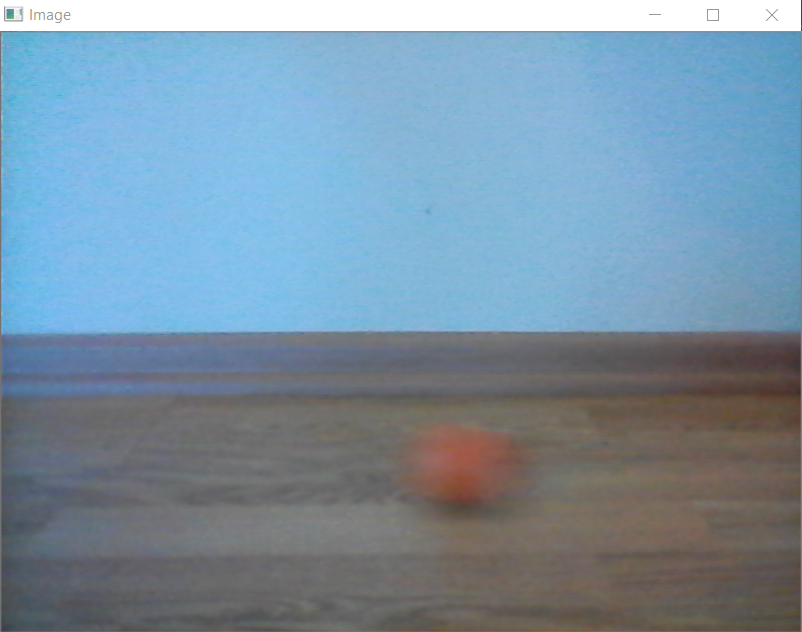
\includegraphics[width=\linewidth]{fig/img1.png}
    \caption{Image captured from video camera.}
  \end{subfigure}
\hspace{0.5cm}
  \begin{subfigure}[b]{0.4\linewidth}
    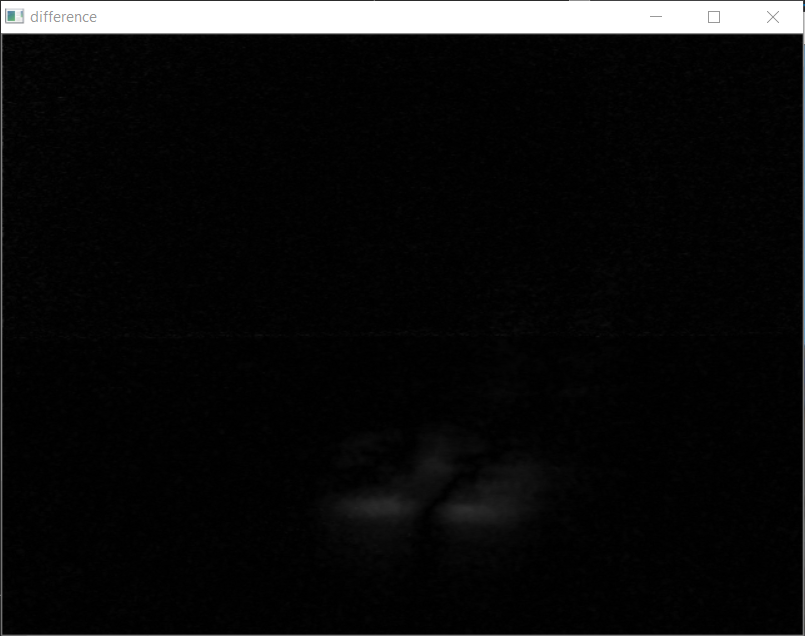
\includegraphics[width=\linewidth]{fig/img2.png}
    \caption{Difference image between 2 frames.}
  \end{subfigure}
	\begin{subfigure}[b]{0.4\linewidth}
    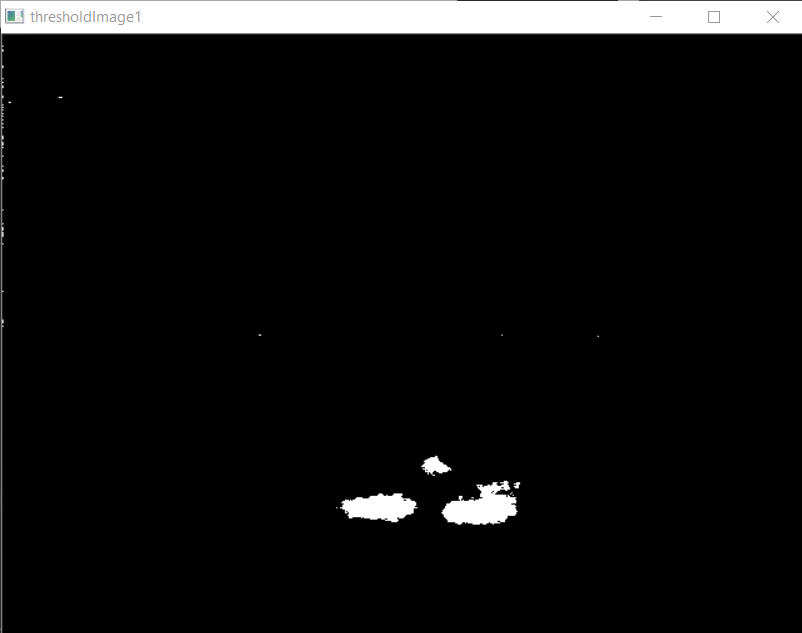
\includegraphics[width=\linewidth]{fig/img3.png}
    \caption{Threshold image.}
  \end{subfigure}
\hspace{0.5cm}
  \begin{subfigure}[b]{0.4\linewidth}
    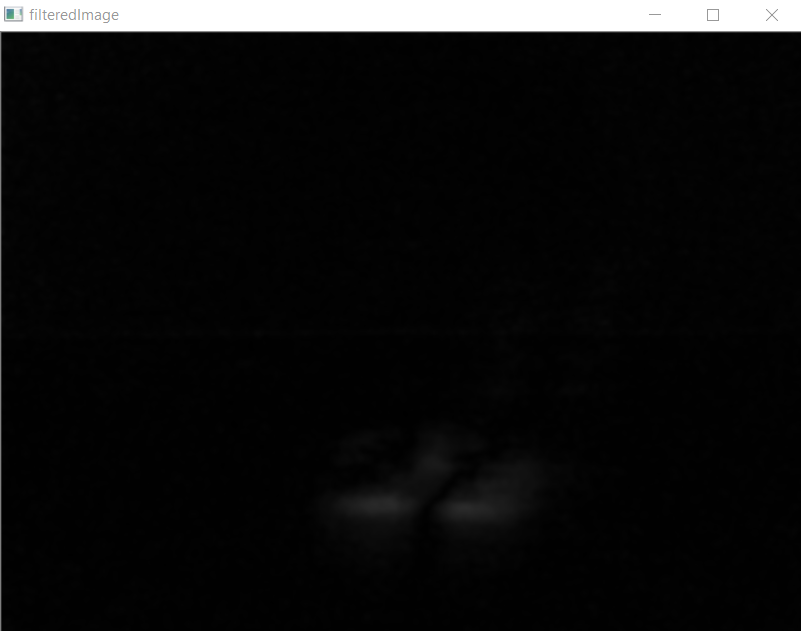
\includegraphics[width=\linewidth]{fig/img4.png}
    \caption{Filtered image.}
  \end{subfigure}
  \begin{subfigure}[b]{0.4\linewidth}
    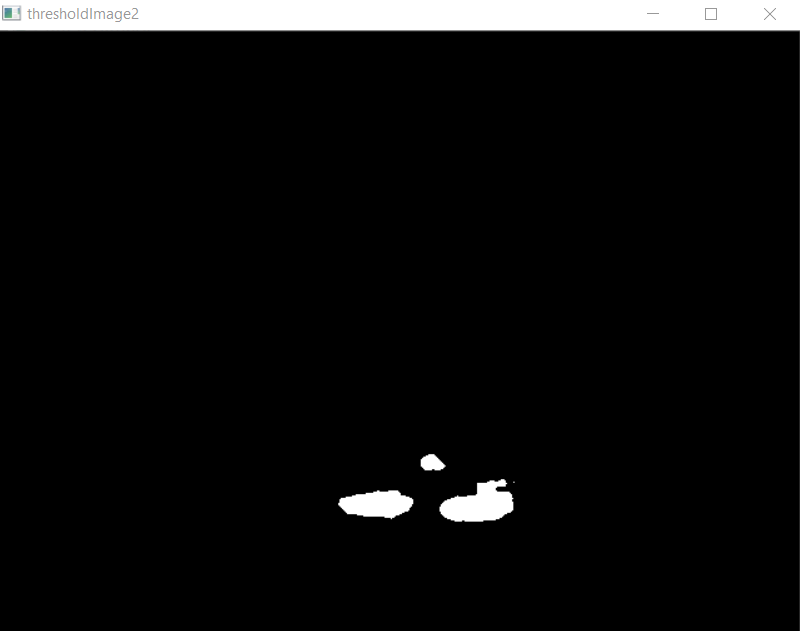
\includegraphics[width=\linewidth]{fig/img5.png}
    \caption{Second threshold image.}
  \end{subfigure}
\hspace{0.5cm}
	\begin{subfigure}[b]{0.4\linewidth}
    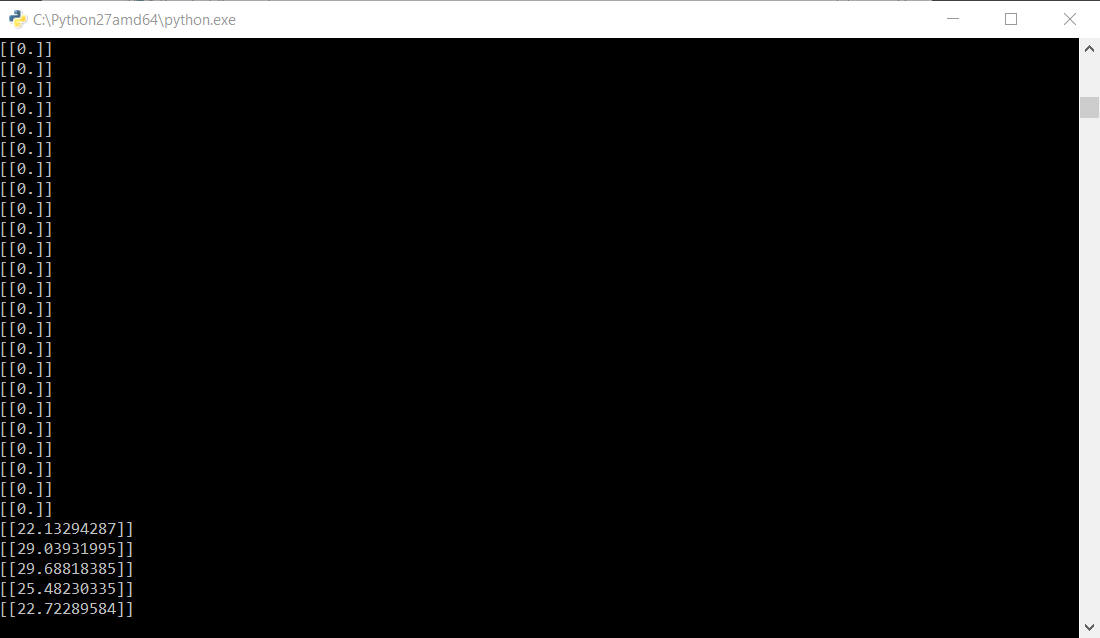
\includegraphics[width=\linewidth]{fig/img6.png}
    \caption{Output of standard deviation.}
  \end{subfigure}
  \caption{Example of program: rolling ball target}
  \label{fig:pic1}
\end{figure}

\vspace{0.5cm}

\section{main.py}
This file deals with the Web app page generation, and is the file that has to be run in order to start the project. 

The Web app has 2 pages: '/' and '/recording' \ref{fig:pic2}, which render 2 different html template files, stored in the \textit{templates} directory. In the html file rendered in the '/recording' file, there is an \textit{img} tag, that has as source the url for another route defined in \textit{main.py}: '/video\_feed'. This method return a Response, containing the frame returned from the VideoCamera class.


\vspace{0.5cm}
\begin{figure}[h!]
  \centering
  \begin{subfigure}[b]{0.4\linewidth}
    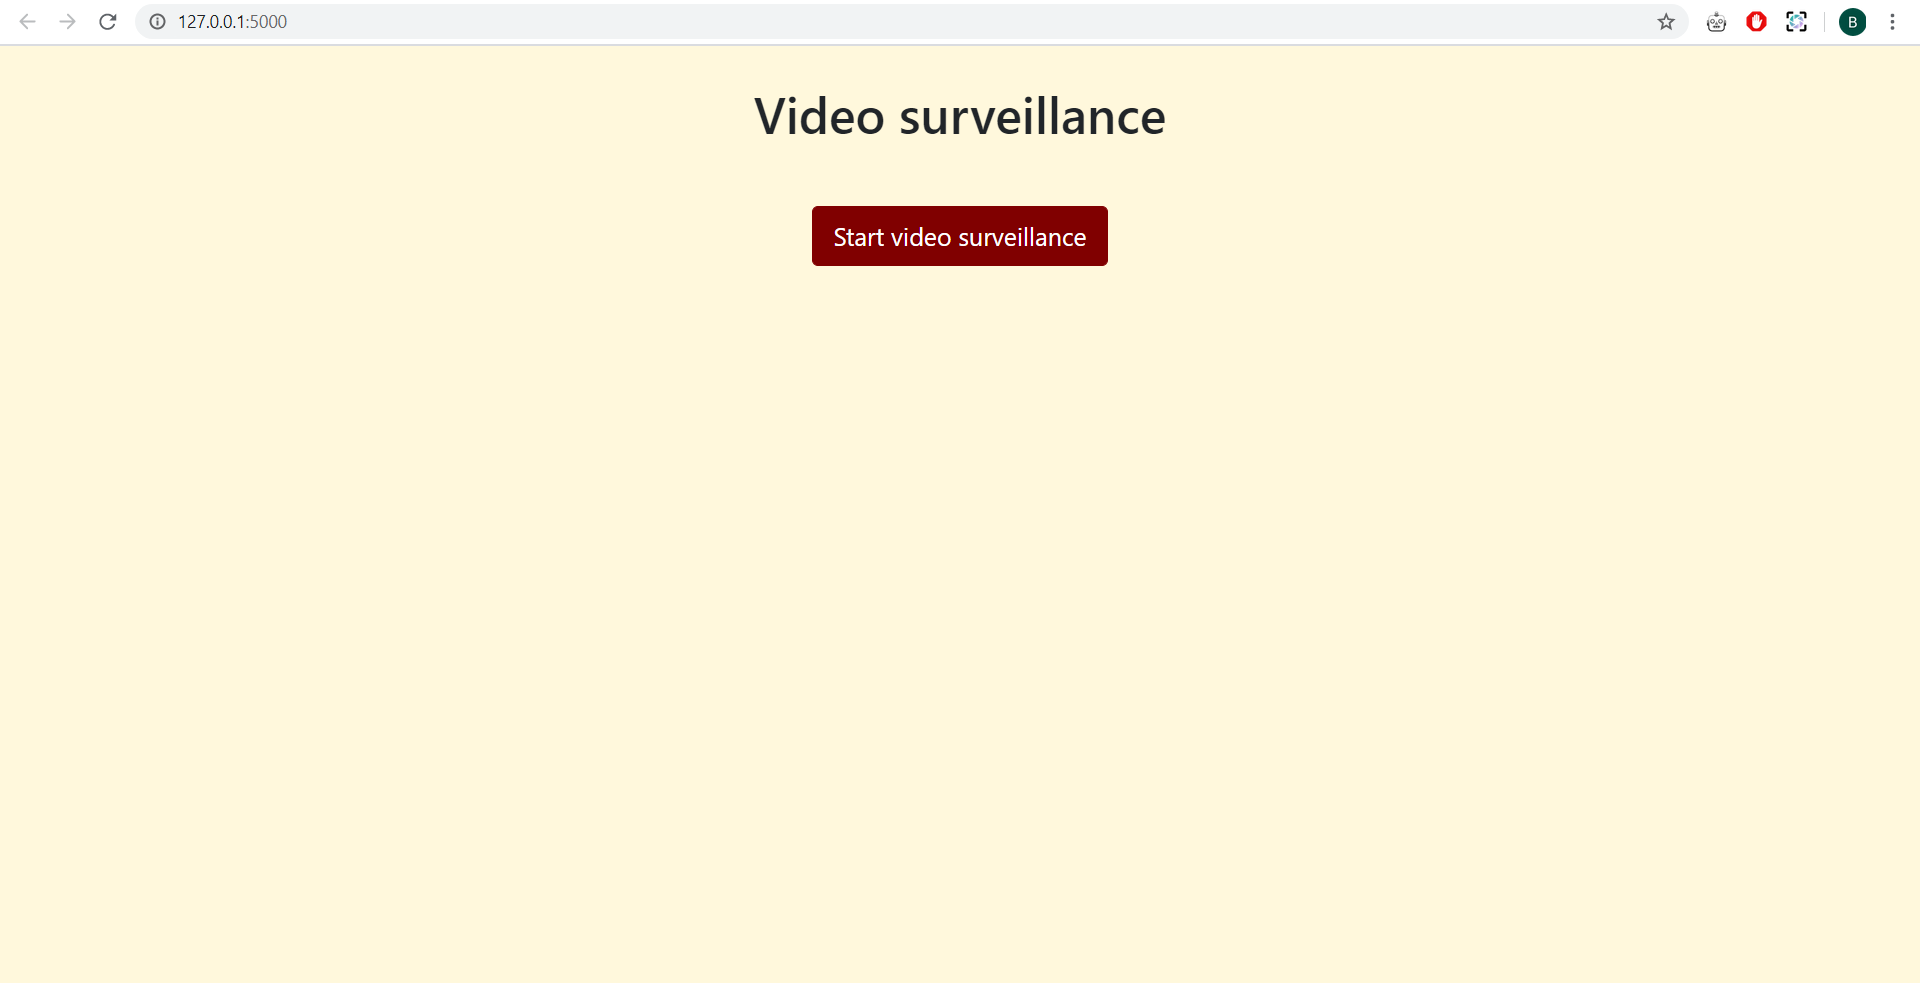
\includegraphics[width=\linewidth]{fig/site1.png}
    \caption{Home page.}
  \end{subfigure}
\hspace{0.5cm}
  \begin{subfigure}[b]{0.4\linewidth}
    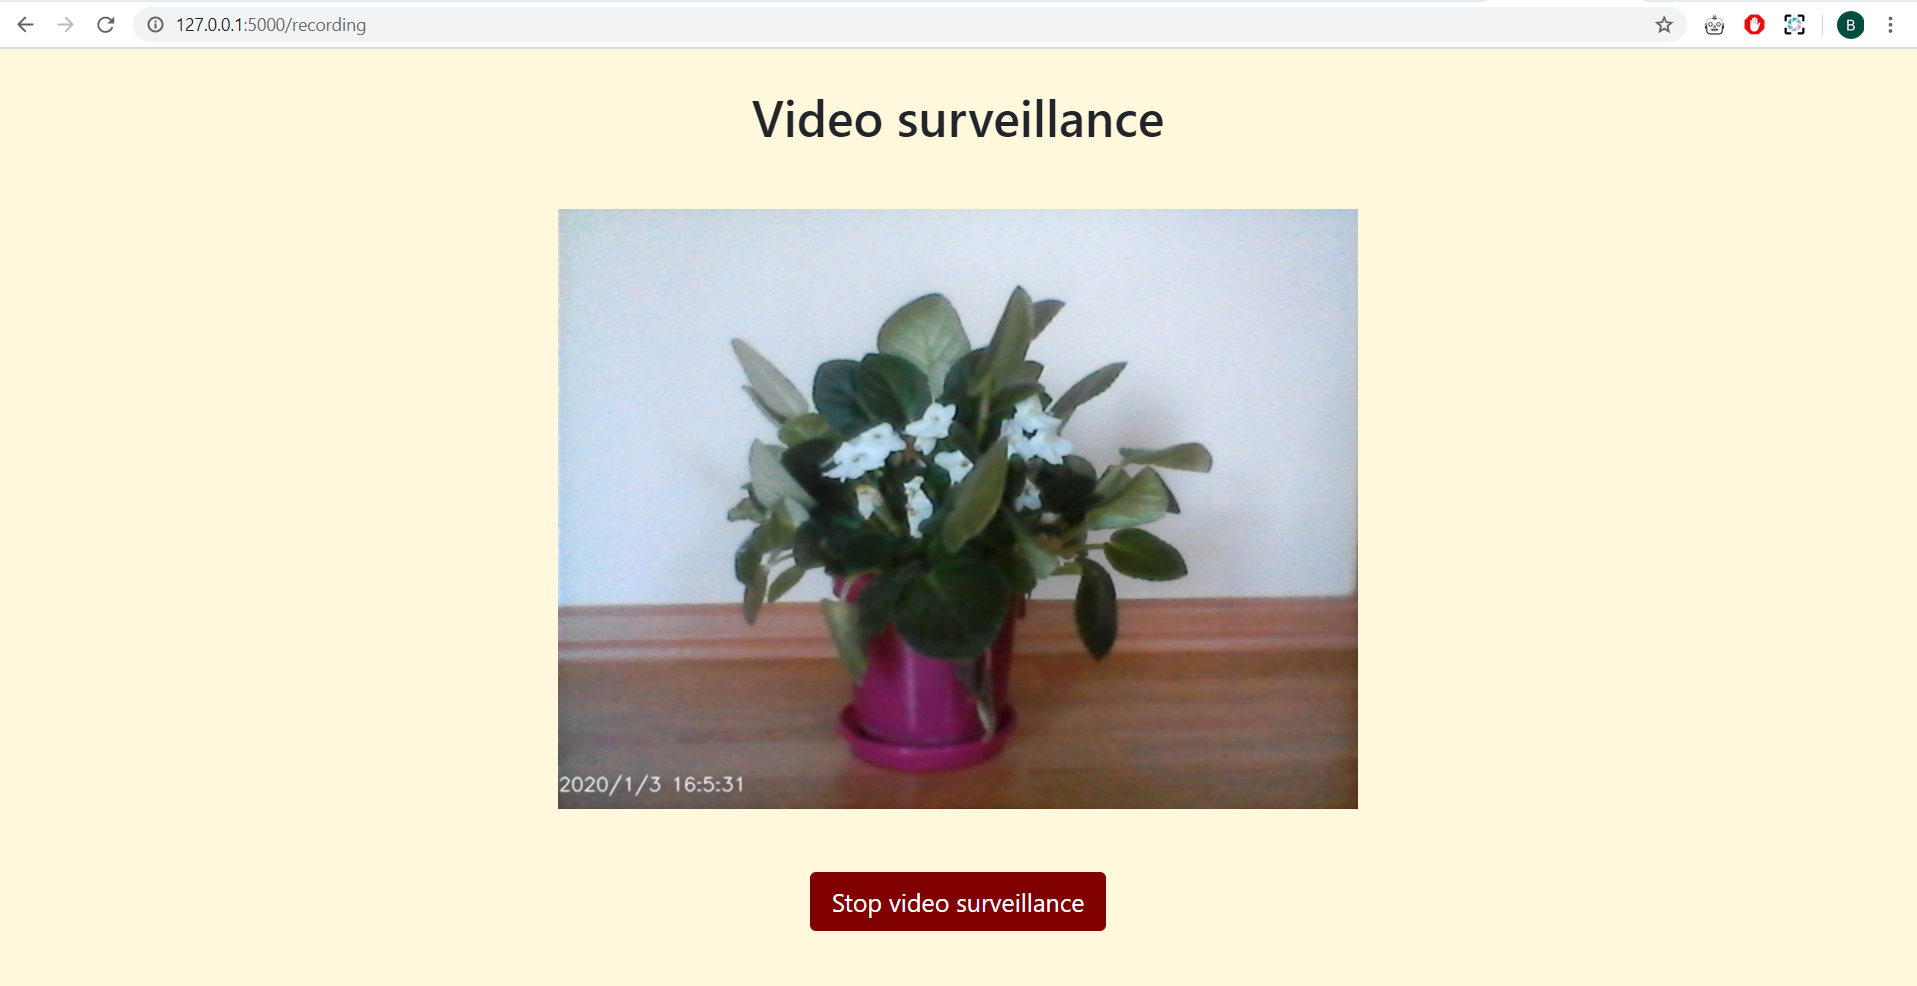
\includegraphics[width=\linewidth]{fig/site2.png}
    \caption{Recording page.}
  \end{subfigure}
  \caption{Web application layout}
  \label{fig:pic2}
\end{figure}

\vspace{0.5cm}


\chapter{Testing and validation}

In regards to the testing of the program, I have run several experiments with it, that generated what I consider to be satisfying results. I have also experimented with different values for the OpenCV functions, that made the system more or less sensitive to movement, and the current configuration I believe to be the best one.

The corectness of this program can also be observed in picture \ref{fig:pic3}, in the output values of the standard deviation. We can see that before the ball started rolling, the frame was a static one, therefore the output was 0. When the ball started rolling, we can see the standard deviation started having positive values.

\vspace{0.5cm}
\begin{figure}[h!]
  \centering
    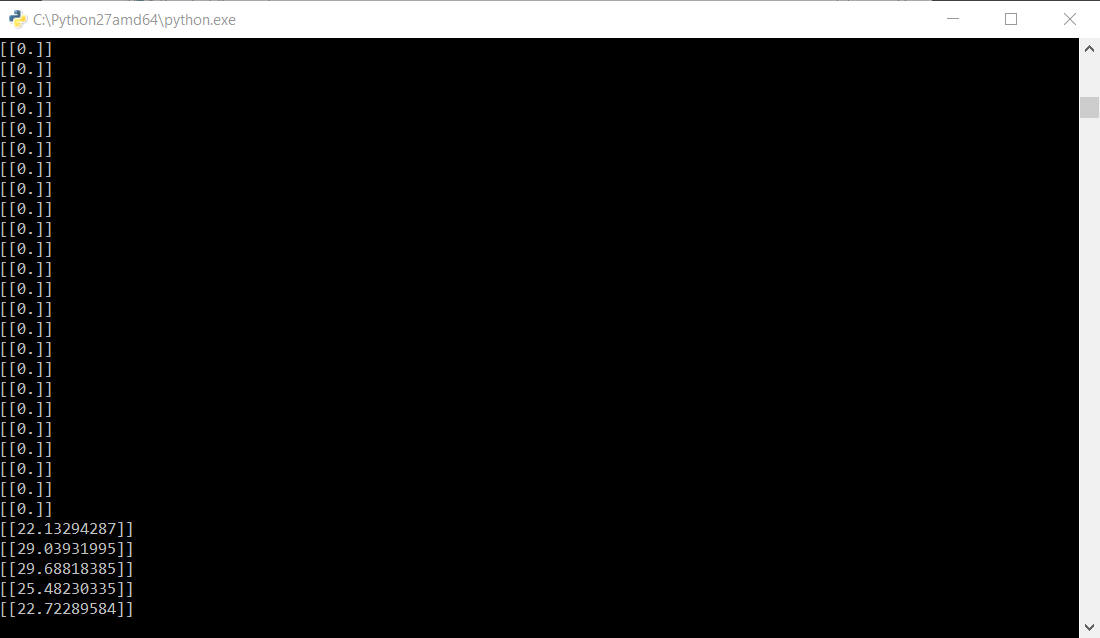
\includegraphics[width=\linewidth]{fig/img6.png}
  \caption{Standard deviation values}
  \label{fig:pic3}
\end{figure}

\vspace{0.5cm}

\bibliographystyle{plain}
\bibliography{is}


\vspace{2cm}
\begin{center}

\includegraphics[width=10cm]{fig/footer}
\end{center}



\end{document}
